\documentclass[tikz,border=0pt]{standalone}
\usepackage[T1]{fontenc}
\usepackage{helvet}
\renewcommand{\familydefault}{\sfdefault}
\usetikzlibrary{arrows.meta,calc}
\newcommand{\markhinge}[2]{\fill (#1,#2) circle (.27mm);}
\tikzset{
 flow/.style={-{Stealth[length=1.7mm,width=1.15mm]},line width=.5pt},
 pics/hingex/.style={code={
   \foreach \i in {-3,-2,-1,0,1,2,3}{
      \markhinge{\i}{.65*\i}\markhinge{\i}{-.65*\i}
   }
   \foreach \i in {-1,0,1}{\markhinge{\i}{.6}\markhinge{\i}{-.6}}
 }},
 pics/hingev/.style={code={
   \foreach \i in {-3,-2,-1,0,1,2,3}{
      \pgfmathsetmacro{\yy}{.5*abs(\i)+.8}
      \markhinge{\i}{\yy}\markhinge{\i}{-\yy}
   }
 }},
 pics/hingevzv/.style={code={
   \foreach \i in {-3,-2,-1,0,1,2,3}{
     \markhinge{\i}{2}\markhinge{\i}{-2}
   }
   \foreach \i in {-1.4,-.7,0,.7,1.4}{
     \markhinge{-2.5}{\i}\markhinge{2.5}{\i}
     \markhinge{-.8}{\i}\markhinge{.8}{\i}
   }
 }},
 pics/hingedxa/.style={code={
   \foreach \i in {-3,-2,-1,0,1,2,3}{
     \markhinge{\i}{.35*\i+.4}\markhinge{\i}{-.2*\i-.4}
     \markhinge{\i}{.35*\i+1.1}
   }
 }},
 pics/hingedxb/.style={code={
   \foreach \i in {-3,-2,-1,0,1,2,3}{
     \markhinge{\i}{-.3*\i+.1}\markhinge{\i}{.2*\i-.5}
     \markhinge{\i}{-.3*\i+1.0}
   }
 }}}
\begin{document}
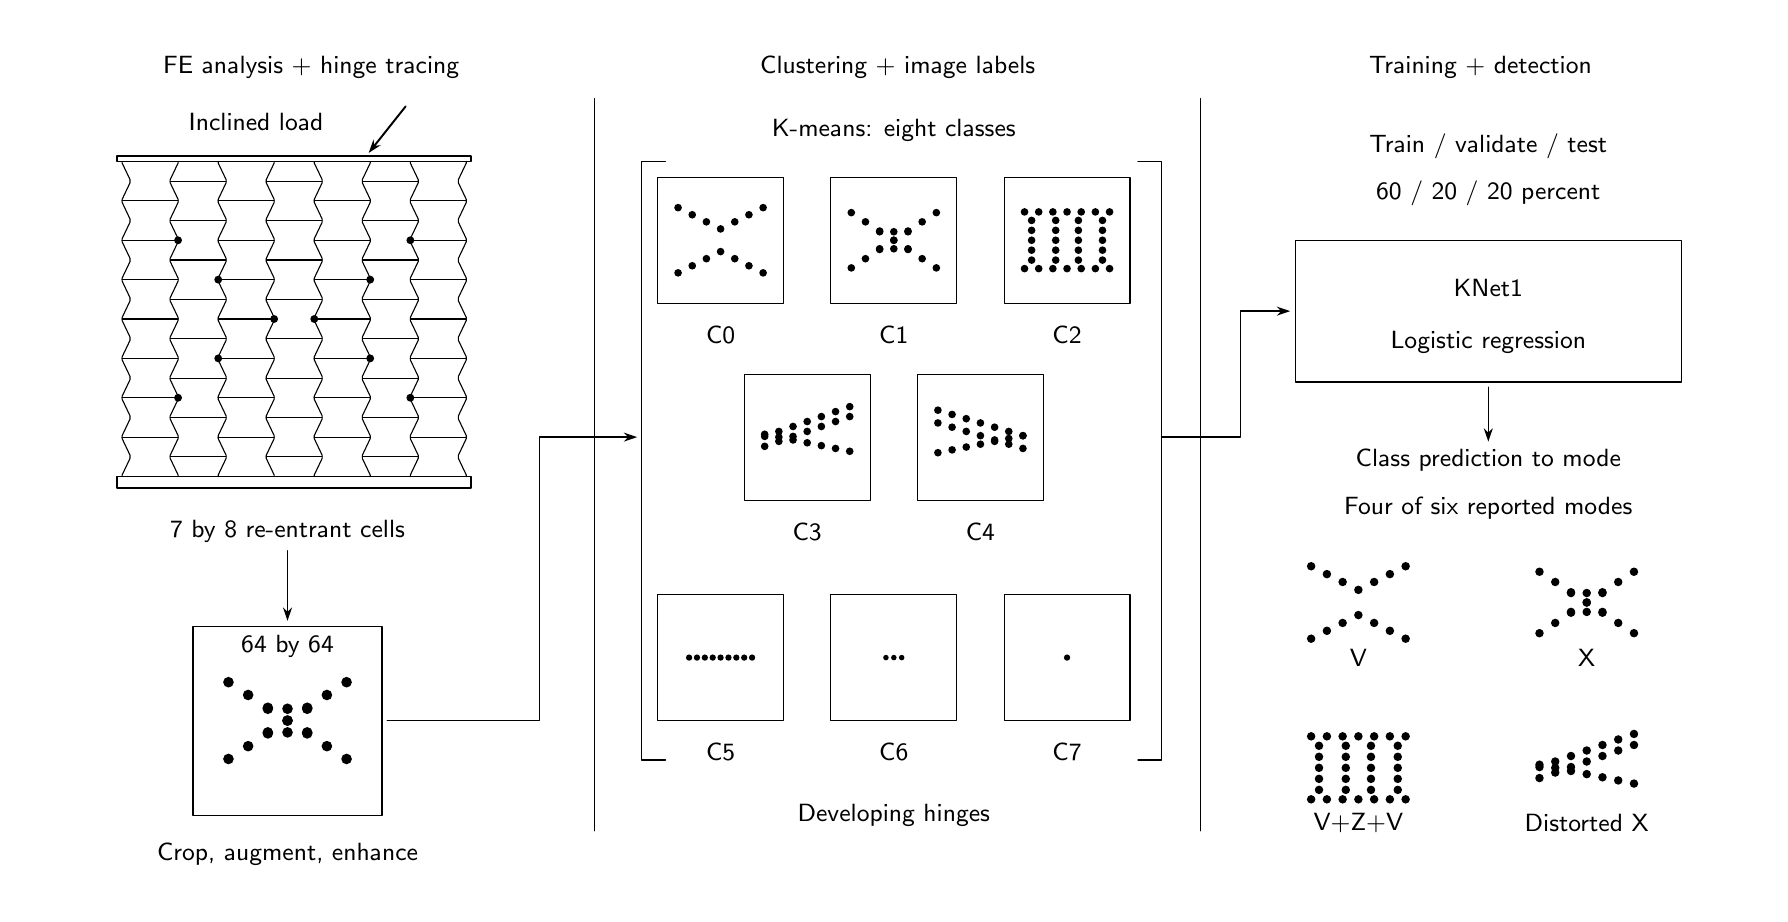
\begin{tikzpicture}[x=1mm,y=1mm,line width=.4pt,line cap=round,line join=round,
 every node/.style={font=\fontsize{9}{11}\selectfont,inner sep=1pt}]
\path[use as bounding box] (0,0) rectangle (220,110);
% Three stages from accepted-manuscript Fig. 3; no simulated data is plotted.
\node at (36,105) {FE analysis + hinge tracing};
\node at (110.5,105) {Clustering + image labels};
\node at (184.5,105) {Training + detection};
\draw (72,101)--(72,8) (149,101)--(149,8);
% Eight alternating wall chains define seven staggered columns of cells.
% P=6.1, H=5, indentation=1: outer/waist widths 7.1/5.1.
% Alternating horizontal ligaments follow accepted Figure 4 connectivity.
\begin{scope}[shift={(12,53)}]
 \foreach \j in {0,...,7}{
   \pgfmathtruncatemacro{\phase}{mod(\j,2)}
   \pgfmathsetmacro{\xb}{6.1*\j+\phase}
   \pgfmathsetmacro{\xm}{6.1*\j+1-\phase}
   \foreach \r in {0,...,7}{
     \draw (\xb,5*\r)--(\xb,5*\r+.2)
       --(\xm,5*\r+2.3)--(\xm,5*\r+2.7)
       --(\xb,5*\r+4.8)--(\xb,5*\r+5);
   }
 }
 % Neighbouring cell columns are offset by half a vertical period.
 \foreach \c in {0,2,4,6}{
   \foreach \r in {0,...,8}{
     \draw (6.1*\c,5*\r)--({6.1*(\c+1)+1},5*\r);
   }
 }
 \foreach \c in {1,3,5}{
   \foreach \r in {0,...,7}{
     \draw (6.1*\c,5*\r+2.5)--({6.1*(\c+1)+1},5*\r+2.5);
   }
 }
 \draw[line width=.7pt] (-.6,-1.5) rectangle (44.3,0);
 \draw[line width=.7pt] (-.6,40) rectangle (44.3,40.7);
 % Mark actual wall joints; these are illustrative, not measured strains.
 \foreach \j/\r in {1/2,6/2,2/3,5/3,3/4,4/4,2/5,5/5,1/6,6/6}{
   \pgfmathtruncatemacro{\phase}{mod(\j,2)}
   \fill (6.1*\j+\phase,5*\r) circle (.5mm);
 }
\end{scope}
\coordinate (load-contact) at (43,93.7);
\draw[flow,line width=.7pt,shorten >=.5mm] (48,100)--(load-contact);
\node at (29,98) {Inclined load};
\node[align=center] (specimen-caption) at (33,46) {7 by 8 re-entrant cells};
% Named image and labels give the process arrows explicit endpoints.
\node[draw,minimum width=24mm,minimum height=24mm,inner sep=0pt]
  (roi) at (33,22) {};
\pic[scale=2.5] at (33,22) {hingex};
\node at (33,31.5) {64 by 64};
\node[align=center] at (33,5) {Crop, augment, enhance};
\draw[flow,shorten <=.6mm,shorten >=.6mm]
  (specimen-caption.south)--(roi.north);
% Five mode-related image classes, as labelled in accepted Table 1.
\foreach \x/\id/\pattern in {88/C0/hingev,110/C1/hingex,132/C2/hingevzv}{
 \draw (\x-8,75) rectangle (\x+8,91);
 \pic[scale=1.8] at (\x,83) {\pattern};
 \node at (\x,71) {\id};
}
\foreach \x/\id/\pattern in {99/C3/hingedxa,121/C4/hingedxb}{
 \draw (\x-8,50) rectangle (\x+8,66);
 \pic[scale=1.8] at (\x,58) {\pattern};
 \node at (\x,46) {\id};
}
\node (cluster-label) at (110,97) {K-means: eight classes};
\draw (81,93)--(78,93)--(78,17)--(81,17);
\coordinate (cluster-input) at (78,58);
\draw[flow,shorten <=.6mm,shorten >=.6mm]
  (roi.east)--(65,22)--(65,58)--(cluster-input);
% Three developing-hinge classes are not additional named modes.
\foreach \x/\id in {88/C5,110/C6,132/C7}{
 \draw (\x-8,22) rectangle (\x+8,38);
 \node at (\x,18) {\id};
}
\foreach \i in {-4,...,4}{\fill (88+\i,30) circle (.4mm);}
\foreach \i in {-1,0,1}{\fill (110+\i,30) circle (.35mm);}
\fill (132,30) circle (.4mm);
\node at (110,10) {Developing hinges};
% Cluster labels train a classifier; inference uses an image separately.
\draw (141,93)--(144,93)--(144,17)--(141,17);
\node[align=center] at (185.5,95) {Train / validate / test};
\node[align=center] at (185.5,89) {60 / 20 / 20 percent};
\node[draw,minimum width=49mm,minimum height=18mm,inner sep=0pt]
  (classifier) at (185.5,74) {};
\node[align=center] at (185.5,77) {KNet1};
\node[align=center] at (185.5,70) {Logistic regression};
\draw[flow,shorten >=.6mm]
  (144,58)--(154,58)--(154,74)--(classifier.west);
\node (prediction) at (185.5,55) {Class prediction to mode};
\draw[flow,shorten <=.6mm,shorten >=.6mm]
  (classifier.south)--(prediction.north);
\node at (185.5,49) {Four of six reported modes};
% The four output modes are hinge fields, not merely letter glyphs.
\foreach \x/\y/\pattern/\name in {169/37/hingev/V,198/37/hingex/X,169/16/hingevzv/V+Z+V,198/16/hingedxa/Distorted X}{
 \pic[scale=2] at (\x,\y) {\pattern};
 \node at (\x,\y-7) {\name};
}
\end{tikzpicture}
\end{document}
